
\documentclass{beamer}
\usepackage[latin1]{inputenc}
%\usetheme{Montpellier}
%\usetheme{Boadilla}
%\usecolortheme[RGB={204,51,255}]{structure}
%\usecolortheme[named=purple]{structure}
\usecolortheme[RGB={62,128,62}]{structure}
%\definecolor{dark}{rgb}{0.3,0.15,0.3}
%\definecolor{light}{rgb}{0.8,0.6,0.8}
%\definecolor{reddish}{rgb}{.5,0.15,0.15}
\definecolor{dark}{rgb}{0.5,0.3,0.4}
%\definecolor{light}{rgb}{0.8,0.6,0.8}
\definecolor{reddish}{rgb}{.7,0.25,0.25}
\definecolor{greenish}{rgb}{.25,0.7,0.25}
\definecolor{blueish}{rgb}{.25,0.25,0.7}
\definecolor{purple}{rgb}{.5,0.0,0.5}
\usepackage{graphicx}
\usepackage{pstricks}

\setbeamertemplate{navigation symbols}{}

\newcommand{\crish}{\color{reddish}}
\newcommand{\cbla}{\color{black}}
\newcommand{\cred}{\color{red}}
\newcommand{\cblu}{\color{blue}}
\newcommand{\cgre}{\color{green}}

\newcommand{\sm}{\color{reddish}$}
\newcommand{\fm}{$\color{black}{}}

\newcommand{\letter}[1]{\color{blue}\texttt{#1}\color{black}}
\newcommand{\binary}[1]{\color{red}\texttt{#1}\color{black}}

\usepackage{tikz}
\usetikzlibrary{arrows,decorations.markings,positioning}
\usepackage{epstopdf}

\title[1d Shannon's Entropy: lecture 2]{1d Shannon's Entropy: lecture 2}
\author{COMSM0075 Information Processing and Brain}
\institute{\texttt{comsm0075.github.io}}
\date{September 2020}

\begin{document}

\maketitle

\begin{frame}{Shannon's entropy}
  For a finite discrete distribution with random variable \sm X\fm,
  possible outcomes \sm\{x_1,x_2,\ldots x_n\}\in\mathcal{X}\fm{} and a
  probability mass function \sm p_X\fm{} giving probabilities \sm p_X(x_i)\fm, the
  entropy is
\crish
  $$
H(X)=-\sum_{x_i\in \mathcal{X}}{p_X(x_i)\log_2p_X(x_i)}
  $$
\cbla
\end{frame}



\begin{frame}{Shannon's entropy}
  For a finite discrete distribution with random variable \sm X\fm,
  possible outcomes \cblu $\{x_1,x_2,\ldots x_n\}\in\mathcal{X}$\cbla{} and a
  probability mass function \sm p_X\fm{} giving probabilities \sm p_X(x_i)\fm, the
  entropy is
\crish
  $$
H(X)=-\sum_{x_i\in \mathcal{X}}{p_X(x_i)\log_2p_X(x_i)}
  $$
\cbla
\end{frame}


\begin{frame}{Shannon's entropy}
  For a finite discrete distribution with random variable \sm X\fm,
  possible outcomes \sm\{x_1,x_2,\ldots x_n\}\in\mathcal{X}\fm{} and a
  probability mass function \sm p_X\fm{} giving probabilities \cblu$ p_X(x_i)$\cbla, the
  entropy is
\crish
  $$
H(X)=-\sum_{x_i\in \mathcal{X}}{p_X(x_i)\log_2p_X(x_i)}
  $$
\cbla
\end{frame}


\begin{frame}{Shannon's entropy}
  For a finite discrete distribution with random variable \sm X\fm,
  possible outcomes \sm\{x_1,x_2,\ldots x_n\}\in\mathcal{X}\fm{} and a
  probability mass function \sm p_X\fm{} giving probabilities \sm p_X(x_i)\fm, the
  entropy is
\crish
  $$
H(X)=-\sum_{x_i\in \mathcal{X}}{p_X(x_i)\log_2p_X(x_i)}
  $$
\cbla
In this definition \sm p\log_2{p}=0\fm{} when \sm p=0\fm; this makes sense since
\crish
$$
\lim_{p\rightarrow 0}p\log_2{p}=0
$$
\cbla

\end{frame}



\begin{frame}{Shannon's entropy}
  For a finite discrete distribution with random variable \sm X\fm,
  possible outcomes \sm\{x_1,x_2,\ldots x_n\}\in\mathcal{X}\fm{} and a
  probability mass function \sm p_X\fm{} giving probabilities \sm p_X(x_i)\fm, the
  entropy is
\crish
  $$
H(X)=-\langle \log_2{p_X(X)}\rangle
  $$
\cbla
\end{frame}


\begin{frame}{Shannon's entropy}
  For a finite discrete distribution with random variable \sm X\fm,
  possible outcomes \sm\{x_1,x_2,\ldots x_n\}\in\mathcal{X}\fm{} and a
  probability mass function \sm p_X\fm{} giving probabilities \sm p_X(x_i)\fm, the
  entropy is
\crish
  $$
H(X)=-\cblu\langle\crish \log_2{p_X(X)}\cblu\rangle\crish
  $$
\cbla
\end{frame}


\begin{frame}{Shannon's entropy}
  \begin{quote}
    Shannon's entropy has lots of nice properties, being easy to estimate isn't one.
  \end{quote}
\end{frame}

\begin{frame}{works on any sample space}
The mean of a distribution
\crish
$$
\langle x\rangle = \sum_{x_i\in \mathcal{X}}{p_X(x_i)x_i}
$$
\cbla
only works if the \sm x\fm s live in a vector space. 
  \end{frame}


\begin{frame}{works on any sample space}
Not all sample spaces are vector spaces, trying to work out the average fruit bought in a grocers doesn't make sense because
\crish
$$
0.25\times \mbox{\color{green}apple\crish}+0.125\times \mbox{\color{yellow}banana\crish}+0.1\times \mbox{\color{orange}orange\crish}\ldots
$$ \cbla is nonsense.
  \end{frame}


\begin{frame}{it's always positive}
\crish
  $$
H(X)=-\sum_{x_i\in \mathcal{X}}{p_X(x_i)\log_2p_X(x_i)}
$$
\cbla
 and since \sm 0\le p_X(x_i)\le 1 \fm 
 \crish
 $$
 H(X)\ge 0
 $$
 \cbla
\end{frame}

\begin{frame}{it's zero if the distribution isn't random}
  If \sm p_X(x_i)\fm{} look like \sm\{0,0,\dots,1,\ldots 0\}\fm{} then
\crish
 $$
 H(X)= 0
 $$
 \cbla
\end{frame}

\begin{frame}{uniform distribution}
  If the distribution is uniform
  \crish
  $$
  p_X(x_i)=\frac{1}{N}
$$
  \cbla
  for all \sm x_i\fm{} where
    \crish
  $$
  N=\#\mathcal{X}
$$
  \cbla
then, since \sm-\log_2(1/N)=log_2{N}\fm{}  
 \crish
 $$
 H(X)=\log_2{N}
 $$
 \cbla
\end{frame}

\begin{frame}{bounds}
  In fact, not proved here but not difficult to prove,
  \crish
  $$
  0\le H(X) \le N
  $$
  \cbla
  with \sm H(X)\fm{} \cblu only\cbla{} if one probability is one and the rest zero and \sm H(X)=N\fm{} \cblu{}only\cbla{} for the uniform distribution.
\end{frame}

\begin{frame}{bounds}
  \crish
  $$
  0\le H(X) \le N
  $$
  \cbla
  That what we want!
  \end{frame}

\begin{frame}{$N=2$}
Two outcomes, \sm a\fm{} and \sm b\fm{} with \sm p(a)=p\fm{} and
\sm{}p(b)=1-p\fm{} then
\crish
$$
H=-p\log_2{p}-(1-p)\log_2{(1-p)}
$$
\cbla
\begin{center}
% GNUPLOT: LaTeX picture with Postscript
\begingroup
  \makeatletter
  \providecommand\color[2][]{%
    \GenericError{(gnuplot) \space\space\space\@spaces}{%
      Package color not loaded in conjunction with
      terminal option `colourtext'%
    }{See the gnuplot documentation for explanation.%
    }{Either use 'blacktext' in gnuplot or load the package
      color.sty in LaTeX.}%
    \renewcommand\color[2][]{}%
  }%
  \providecommand\includegraphics[2][]{%
    \GenericError{(gnuplot) \space\space\space\@spaces}{%
      Package graphicx or graphics not loaded%
    }{See the gnuplot documentation for explanation.%
    }{The gnuplot epslatex terminal needs graphicx.sty or graphics.sty.}%
    \renewcommand\includegraphics[2][]{}%
  }%
  \providecommand\rotatebox[2]{#2}%
  \@ifundefined{ifGPcolor}{%
    \newif\ifGPcolor
    \GPcolorfalse
  }{}%
  \@ifundefined{ifGPblacktext}{%
    \newif\ifGPblacktext
    \GPblacktexttrue
  }{}%
  % define a \g@addto@macro without @ in the name:
  \let\gplgaddtomacro\g@addto@macro
  % define empty templates for all commands taking text:
  \gdef\gplbacktext{}%
  \gdef\gplfronttext{}%
  \makeatother
  \ifGPblacktext
    % no textcolor at all
    \def\colorrgb#1{}%
    \def\colorgray#1{}%
  \else
    % gray or color?
    \ifGPcolor
      \def\colorrgb#1{\color[rgb]{#1}}%
      \def\colorgray#1{\color[gray]{#1}}%
      \expandafter\def\csname LTw\endcsname{\color{white}}%
      \expandafter\def\csname LTb\endcsname{\color{black}}%
      \expandafter\def\csname LTa\endcsname{\color{black}}%
      \expandafter\def\csname LT0\endcsname{\color[rgb]{1,0,0}}%
      \expandafter\def\csname LT1\endcsname{\color[rgb]{0,1,0}}%
      \expandafter\def\csname LT2\endcsname{\color[rgb]{0,0,1}}%
      \expandafter\def\csname LT3\endcsname{\color[rgb]{1,0,1}}%
      \expandafter\def\csname LT4\endcsname{\color[rgb]{0,1,1}}%
      \expandafter\def\csname LT5\endcsname{\color[rgb]{1,1,0}}%
      \expandafter\def\csname LT6\endcsname{\color[rgb]{0,0,0}}%
      \expandafter\def\csname LT7\endcsname{\color[rgb]{1,0.3,0}}%
      \expandafter\def\csname LT8\endcsname{\color[rgb]{0.5,0.5,0.5}}%
    \else
      % gray
      \def\colorrgb#1{\color{black}}%
      \def\colorgray#1{\color[gray]{#1}}%
      \expandafter\def\csname LTw\endcsname{\color{white}}%
      \expandafter\def\csname LTb\endcsname{\color{black}}%
      \expandafter\def\csname LTa\endcsname{\color{black}}%
      \expandafter\def\csname LT0\endcsname{\color{black}}%
      \expandafter\def\csname LT1\endcsname{\color{black}}%
      \expandafter\def\csname LT2\endcsname{\color{black}}%
      \expandafter\def\csname LT3\endcsname{\color{black}}%
      \expandafter\def\csname LT4\endcsname{\color{black}}%
      \expandafter\def\csname LT5\endcsname{\color{black}}%
      \expandafter\def\csname LT6\endcsname{\color{black}}%
      \expandafter\def\csname LT7\endcsname{\color{black}}%
      \expandafter\def\csname LT8\endcsname{\color{black}}%
    \fi
  \fi
  \setlength{\unitlength}{0.0500bp}%
  \begin{picture}(5040.00,3528.00)%
    \gplgaddtomacro\gplbacktext{%
      \csname LTb\endcsname%
      \put(946,704){\makebox(0,0)[r]{\strut{} 0}}%

      \put(946,1216){\makebox(0,0)[r]{\strut{} 0.2}}%

      \put(946,1728){\makebox(0,0)[r]{\strut{} 0.4}}%

      \put(946,2239){\makebox(0,0)[r]{\strut{} 0.6}}%

      \put(946,2751){\makebox(0,0)[r]{\strut{} 0.8}}%

      \put(946,3263){\makebox(0,0)[r]{\strut{} 1}}%
      \put(1078,484){\makebox(0,0){\strut{} 0}}%
      \put(1791,484){\makebox(0,0){\strut{} 0.2}}%
      \put(2504,484){\makebox(0,0){\strut{} 0.4}}%
      \put(3217,484){\makebox(0,0){\strut{} 0.6}}%
      \put(3930,484){\makebox(0,0){\strut{} 0.8}}%
      \put(4643,484){\makebox(0,0){\strut{} 1}}%
      \put(176,1983){\rotatebox{-270}{\makebox(0,0){\strut{}H(X)}}}%
      \put(2860,154){\makebox(0,0){\strut{}$p$}}%
    }%
    \gplgaddtomacro\gplfronttext{%
    }%
    \gplbacktext
    \put(0,0){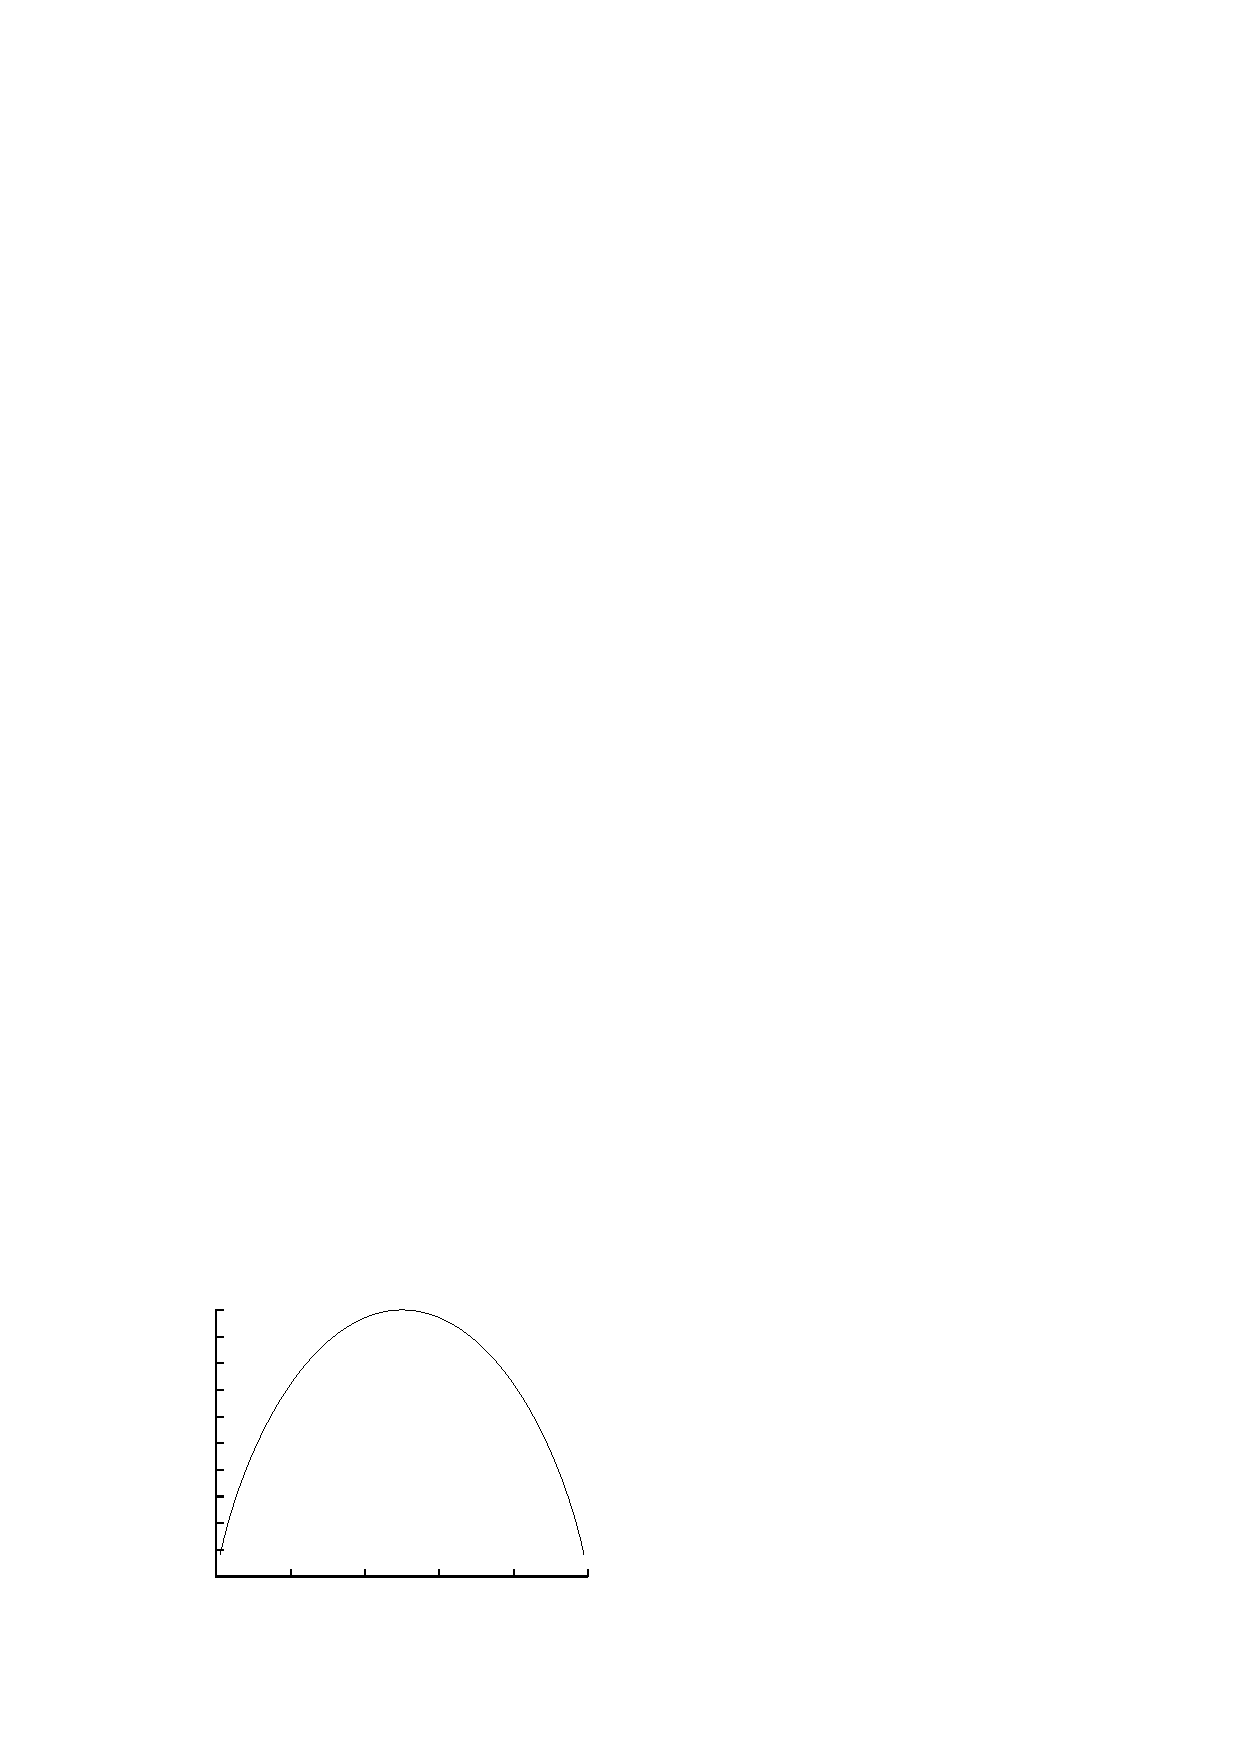
\includegraphics{fig_info_one_d}}%
    \gplfronttext
  \end{picture}%
\endgroup

\end{center}
\end{frame}

\begin{frame}{source coding}
  \begin{quote}
    The main reason to believe that Shannon's entropy is a good
quantity for calculating entropy is its relationship with what is
called source coding.
  \end{quote}
\end{frame}

\begin{frame}{source coding}
  Imagine storing a long sequence of the letters \letter{A}, \letter{B}, \letter{C} and \letter{D} as binary.
  \begin{quote}
    \letter{AABACBDA}$\ldots$
    \end{quote}
\end{frame}

\begin{frame}{a dictionary might look like}
\begin{center}
\begin{tabular}{cccc}
\letter{A}&\letter{B}&\letter{C}&\letter{D}\\
\hline\cred
00&01&\cred 10&\cred 11
\cbla\end{tabular}
\end{center}
\end{frame}


\begin{frame}{a dictionary might look like}
\begin{center}
\begin{tabular}{cccc}
\letter{A}&\letter{B}&\letter{C}&\letter{D}\\
\hline\cred
00&\cred 01&\cred 10&\cred 11
\cbla\end{tabular}
\end{center}
  \begin{quote}
    \letter{AABACD}$\ldots$
  \end{quote}
  becomes
    \begin{quote}
    \binary{000001001011}$\ldots$
    \end{quote}
\end{frame}


\begin{frame}{a dictionary might look like}
\begin{center}
\begin{tabular}{cccc}
\letter{A}&\letter{B}&\letter{C}&\letter{D}\\
\hline\cred
00&\cred 01&\cred 10&\cred 11
\cbla\end{tabular}
\end{center}
  \begin{quote}
    \letter{\cgre A\cblu{}ABACD}$\ldots$
  \end{quote}
  becomes
    \begin{quote}
    \binary{\cgre 00\cred{}0001001011}$\ldots$
    \end{quote}
\end{frame}


\begin{frame}{a dictionary might look like}
\begin{center}
\begin{tabular}{cccc}
\letter{A}&\letter{B}&\letter{C}&\letter{D}\\
\hline\cred
00&\cred 01&\cred 10&\cred 11
\cbla\end{tabular}
\end{center}
  \begin{quote}
    \letter{A\cgre A\cblu{}BACD}$\ldots$
  \end{quote}
  becomes
    \begin{quote}
    \binary{00\cgre 00\cred{}01001011}$\ldots$
    \end{quote}
\end{frame}


\begin{frame}{a dictionary might look like}
\begin{center}
\begin{tabular}{cccc}
\letter{A}&\letter{B}&\letter{C}&\letter{D}\\
\hline\cred
00&\cred 01&\cred 10&\cred 11
\cbla\end{tabular}
\end{center}
  \begin{quote}
    \letter{AA\cgre B\cblu{}ACD}$\ldots$
  \end{quote}
  becomes
    \begin{quote}
    \binary{0000\cgre 01\cred{}001011}$\ldots$
    \end{quote}
\end{frame}


\begin{frame}{a dictionary might look like}
\begin{center}
\begin{tabular}{cccc}
\letter{A}&\letter{B}&\letter{C}&\letter{D}\\
\hline\cred
00&\cred 01&\cred 10&\cred 11
\cbla\end{tabular}
\end{center}
  \begin{quote}
    \letter{AAB\cgre A\cblu{}CD}$\ldots$
  \end{quote}
  becomes
    \begin{quote}
    \binary{000001\cgre 00\cred{}1011}$\ldots$
    \end{quote}
\end{frame}



\begin{frame}{a dictionary might look like}
\begin{center}
\begin{tabular}{cccc}
\letter{A}&\letter{B}&\letter{C}&\letter{D}\\
\hline\cred
00&\cred 01&\cred 10&\cred 11
\cbla\end{tabular}
\end{center}
  \begin{quote}
    \letter{AABA\cgre C\cblu{}D}$\ldots$
  \end{quote}
  becomes
    \begin{quote}
    \binary{00000100\cgre 10\cred{}11}$\ldots$
    \end{quote}
\end{frame}


\begin{frame}{a dictionary might look like}
\begin{center}
\begin{tabular}{cccc}
\letter{A}&\letter{B}&\letter{C}&\letter{D}\\
\hline\cred
00&\cred 01&\cred 10&\cred 11
\cbla\end{tabular}
\end{center}
  \begin{quote}
    \letter{AABAC\cgre D\cblu{}}$\ldots$
  \end{quote}
  becomes
    \begin{quote}
    \binary{0000010010\cgre 11\cred{}}$\ldots$
    \end{quote}
\end{frame}


\begin{frame}{a dictionary might look like}
\begin{center}
\begin{tabular}{cccc}
\letter{A}&\letter{B}&\letter{C}&\letter{D}\\
\hline\cred
00&\cred 01&\cred 10&\cred 11
\cbla\end{tabular}
\end{center}
  \begin{quote}
    \letter{AABACD}$\ldots$
  \end{quote}
  becomes
    \begin{quote}
    \binary{000001001011}$\ldots$
    \end{quote}
\end{frame}

\begin{frame}{average bits per letter}
  \crish
  $$
  L=2
  $$
  \cbla
\end{frame}


\begin{frame}{say we know the letter frequencies}
  Now, say we also knew that
  \begin{center}
\begin{tabular}{cccc}
\letter{A}&\letter{B}&\letter{C}&\letter{D}\\
\hline\cred
0.5&\cred 0.25&\cred 0.125&\cred 0.125
\cbla\end{tabular}
\end{center}
So in the message that will be encoded, \letter{A}{} occurs half the
time, \letter{B}{} a quarter the time and \letter{C}{} and \letter{D}{} an
eighth of the time.
\end{frame}



\begin{frame}{say we know the letter frequencies}

\begin{quote}
  \cred Can we use this information to make \sm L\fm\cred{} smaller?\cbla
  \end{quote}
\end{frame}


\begin{frame}{say we know the letter frequencies}

\begin{quote}
  \cred
  Can we find an shorter encoding for the most frequent letter: \letter{A}?\cbla
  \end{quote}
\end{frame}


\begin{frame}{here is a better code}
\begin{center}
\begin{tabular}{cccc}
\letter{A}&\letter{B}&\letter{C}&\letter{D}\\
\hline
\binary{0}&\binary{10}&\binary{110}&\binary{111}
\end{tabular}
\end{center}
\end{frame}  

\begin{frame}{here is a better code}
\begin{center}
\begin{tabular}{cccc}
\letter{A}&\letter{B}&\letter{C}&\letter{D}\\
\hline
\binary{0}&\binary{10}&\binary{110}&\binary{111}
\end{tabular}
\end{center}
  \begin{quote}
    \letter{AABACD}$\ldots$
  \end{quote}
  becomes
    \begin{quote}
    \binary{00100110111}$\ldots$
    \end{quote}
\end{frame}  

\begin{frame}{here is a better code}
\begin{center}
\begin{tabular}{cccc}
\letter{A}&\letter{B}&\letter{C}&\letter{D}\\
\hline
\binary{0}&\binary{10}&\binary{110}&\binary{111}
\end{tabular}
\end{center}
  \begin{quote}
    \letter{\cgre A\cblu{}ABACD}$\ldots$
  \end{quote}
  becomes
    \begin{quote}
    \binary{\cgre 0\cred{}0100110111}$\ldots$
    \end{quote}
\end{frame}  


\begin{frame}{here is a better code}
\begin{center}
\begin{tabular}{cccc}
\letter{A}&\letter{B}&\letter{C}&\letter{D}\\
\hline
\binary{0}&\binary{10}&\binary{110}&\binary{111}
\end{tabular}
\end{center}
  \begin{quote}
    \letter{A\cgre A\cblu{}BACD}$\ldots$
  \end{quote}
  becomes
    \begin{quote}
    \binary{0\cgre 0\cred{}100110111}$\ldots$
    \end{quote}
\end{frame}  

\begin{frame}{here is a better code}
\begin{center}
\begin{tabular}{cccc}
\letter{A}&\letter{B}&\letter{C}&\letter{D}\\
\hline
\binary{0}&\binary{10}&\binary{110}&\binary{111}
\end{tabular}
\end{center}
  \begin{quote}
    \letter{AA\cgre B\cblu{}ACD}$\ldots$
  \end{quote}
  becomes
    \begin{quote}
    \binary{00\cgre 10\cred{}0110111}$\ldots$
    \end{quote}
\end{frame}  


\begin{frame}{here is a better code}
\begin{center}
\begin{tabular}{cccc}
\letter{A}&\letter{B}&\letter{C}&\letter{D}\\
\hline
\binary{0}&\binary{10}&\binary{110}&\binary{111}
\end{tabular}
\end{center}
  \begin{quote}
    \letter{AAB\cgre A\cblu{}CD}$\ldots$
  \end{quote}
  becomes
    \begin{quote}
    \binary{0010\cgre 0\cred{}110111}$\ldots$
    \end{quote}
\end{frame}  


\begin{frame}{here is a better code}
\begin{center}
\begin{tabular}{cccc}
\letter{A}&\letter{B}&\letter{C}&\letter{D}\\
\hline
\binary{0}&\binary{10}&\binary{110}&\binary{111}
\end{tabular}
\end{center}
  \begin{quote}
    \letter{AABA\cgre C\cblu{}D}$\ldots$
  \end{quote}
  becomes
    \begin{quote}
    \binary{00100\cgre 110\cred{}111}$\ldots$
    \end{quote}
\end{frame}  


\begin{frame}{here is a better code}
\begin{center}
\begin{tabular}{cccc}
\letter{A}&\letter{B}&\letter{C}&\letter{D}\\
\hline
\binary{0}&\binary{10}&\binary{110}&\binary{111}
\end{tabular}
\end{center}
  \begin{quote}
    \letter{AABAC\cgre D\cblu{}}$\ldots$
  \end{quote}
  becomes
    \begin{quote}
    \binary{00100110\cgre 111\cred{}}$\ldots$
    \end{quote}
\end{frame}  


\end{document}


